\documentclass[12pt]{article}

\usepackage{type1ec}
\usepackage{mathtext}
\usepackage[T1, T2A]{fontenc}
\usepackage[utf8]{inputenc}
\usepackage[english, ukrainian]{babel}
\usepackage{amsmath}
\usepackage{amssymb}
\usepackage{amsthm}
\usepackage{xcolor}
\usepackage{graphicx}
\usepackage{listings}
\graphicspath{ {images/} }


\usepackage{geometry}
\geometry{
    a4paper,
    left = 30mm,
    top = 20mm,
    right = 10mm,
    bottom = 20mm
}

\begin{document}
    \pagestyle{empty}

\begin{titlepage}
    \begin{center}

        \textbf{НАЦІОНАЛЬНИЙ ТЕХНІЧНИЙ УНІВЕРСИТЕТ УКРАЇНИ}\\
        “КИЇВСЬКИЙ ПОЛІТЕХНІЧНИЙ ІНСТИТУТ ім. Ігоря Сікорського”\\
        Навчально-науковий фізико-технічний інститут\\
        Кафедра математичних методів захисту інформації

        \vspace{6cm}

        \Large \textbf{Симетрична Криптографія}\\
        Комп'ютерний практикум №1

    \end{center}

    \vspace{9cm}
    \begin{flushright}
        Виконали:\\
        Студенти групи ФІ-13\\
        Ісаченко Нікіта\\
        Бондаренко Олександр
    \end{flushright}

    \vspace*{3cm}

    \begin{center}
        2024 р.
    \end{center}
\end{titlepage}

    \section{Мета роботи}

    Засвоєння понять ентропії на символ джерела та його надлишковості, вивчення та
    порівняння різних моделей джерела відкритого тексту для наближеного визначення
    ентропії, набуття практичних навичок щодо оцінки ентропії на символ джерела.

    \section{Хід роботи}

    Необхідно було підрахувати частоти біграм(як з пробілами, так і без), символів, а також їх ентропій.
    Оскільки реалізовували ми все на мові програмування C++, ми викорстали усю силу потоків стандартної
    бібліотеки цієї мови для обробки текстових файлів. Як кодування взяли застаріле CP-1251, через те,
    що воно вміщуєтся у один байт, і таким чином з ним і простіше працювати(на відміну від utf-8, яке символи в якій можуть кодуватись
    різною довжиною), а також дозволило зменшити обсяг вхідних файлів. Особливих труднощів під час виконання комп'ютерного
    практикуму не виявлено. 

    \section{Результати}

    Оскільки біграм дуже багато, ми взяли відносно невеликий текст, щоб не роздувати звіт на 100 сторінок статистичних даних.

    Нижче наведенинй підрахунок ймовірностей та частот символів у тектсі з пробілами, з відповідним значенням ентропії:

    \begin{verbatim}
        Letters: 
        а -- 71, 0.0527489,
        б -- 19, 0.0141159,
        в -- 62, 0.0460624,
        г -- 18, 0.013373,
        д -- 31, 0.0230312,
        е -- 98, 0.0728083,
        ж -- 18, 0.013373,
        з -- 18, 0.013373,
        и -- 112, 0.0832095,
        й -- 9, 0.00668648,
        к -- 29, 0.0215453,
        л -- 33, 0.0245171,
        м -- 51, 0.03789,
        н -- 83, 0.0616642,
        о -- 125, 0.0928678,
        п -- 25, 0.0185736,
        р -- 51, 0.03789,
        с -- 62, 0.0460624,
        т -- 74, 0.0549777,
        у -- 26, 0.0193165,
        ф -- 1, 0.000742942,
        х -- 15, 0.0111441,
        ц -- 4, 0.00297177,
        ч -- 14, 0.0104012,
        ш -- 2, 0.00148588,
        щ -- 2, 0.00148588,
        ы -- 26, 0.0193165,
        ь -- 32, 0.0237741,
        э -- 3, 0.00222883,
        ю -- 9, 0.00668648,
        я -- 28, 0.0208024,
          -- 195, 0.144874,
        
        Total letter in text: 32
        Entropy of symbols: 4.36575
        
    \end{verbatim}

    Перша колонка- кількість, друга- ймовірність появи. Внизу наведено потужність алфавіту на ентропію на символ(або $H_1$).

    Без пробілів:

    \begin{verbatim}
        Text size: 1151
        Letters: 
        а -- 71, 0.0616855,
        б -- 19, 0.0165074,
        в -- 62, 0.0538662,
        г -- 18, 0.0156386,
        д -- 31, 0.0269331,
        е -- 98, 0.0851434,
        ж -- 18, 0.0156386,
        з -- 18, 0.0156386,
        и -- 112, 0.0973067,
        й -- 9, 0.00781929,
        к -- 29, 0.0251955,
        л -- 33, 0.0286707,
        м -- 51, 0.0443093,
        н -- 83, 0.0721112,
        о -- 125, 0.108601,
        п -- 25, 0.0217202,
        р -- 51, 0.0443093,
        с -- 62, 0.0538662,
        т -- 74, 0.0642919,
        у -- 26, 0.0225891,
        ф -- 1, 0.00086881,
        х -- 15, 0.0130321,
        ц -- 4, 0.00347524,
        ч -- 14, 0.0121633,
        ш -- 2, 0.00173762,
        щ -- 2, 0.00173762,
        ы -- 26, 0.0225891,
        ь -- 32, 0.0278019,
        э -- 3, 0.00260643,
        ю -- 9, 0.00781929,
        я -- 28, 0.0243267,

        Total letter in text: 31
        Entropy of symbols: 4.40741

    \end{verbatim}

    Можемо побачити, що у тексті з пробілами ентропія на символ трохи менша через те, що пробіл -- найчастіший символ,
    що робить розподіл символів менш подібним до випадкового.

    Лістинг підрахунку біграм буде наведений після висновку у додатку А, через його великий об'єм. Однак можемо навести
    результати підрахунку частот та кількостей біграм у тексті.

    З пробілами(перетинні):

    \begin{verbatim}
        Total overlaping bigrams in text: 1345
        Entropy of overlaping bigrams in text: 3.78871
    \end{verbatim}

    З пробілами(неперетинні):
    \begin{verbatim}
        Total non overlaping bigrams in text: 673
        Entropy of non overlaping bigrams in text: 3.66332
    \end{verbatim}

    Без пробілів(перетинні):

    \begin{verbatim}
        Total overlaping bigrams in text: 1150
        Entropy of overlaping bigrams in text: 3.88691
    \end{verbatim}

    Без пробілів(неперетинні):

    \begin{verbatim}
        Total non overlaping bigrams in text: 575
        Entropy of non overlaping bigrams in text: 3.74531
    \end{verbatim}

    \section{Оцінки для $H^{(10)}, H^{(20)}, H^{(30)}$}

    Скріншот підрахунку ентропії $H^{(10)}$ з-за допомогою \textit{CoolPinkProgram}.

    \begin{center}
        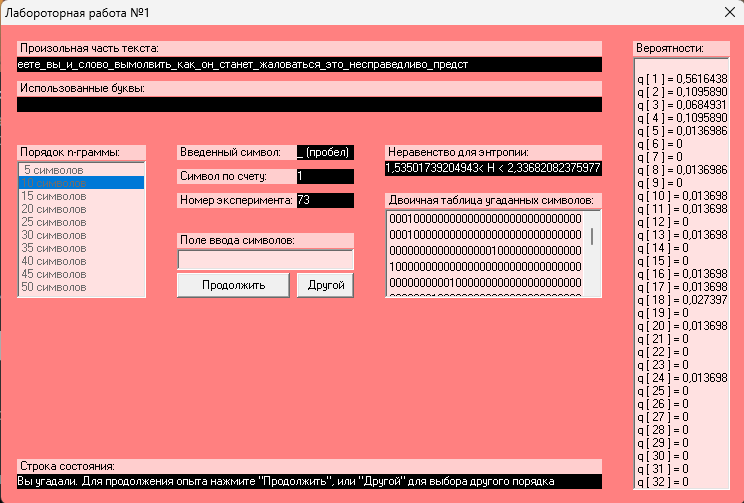
\includegraphics[scale=0.6]{Ентропія 10-грами.png}
    \end{center}

    Скріншот підрахунку ентропії $H^{(20)}$:

    \begin{center}
        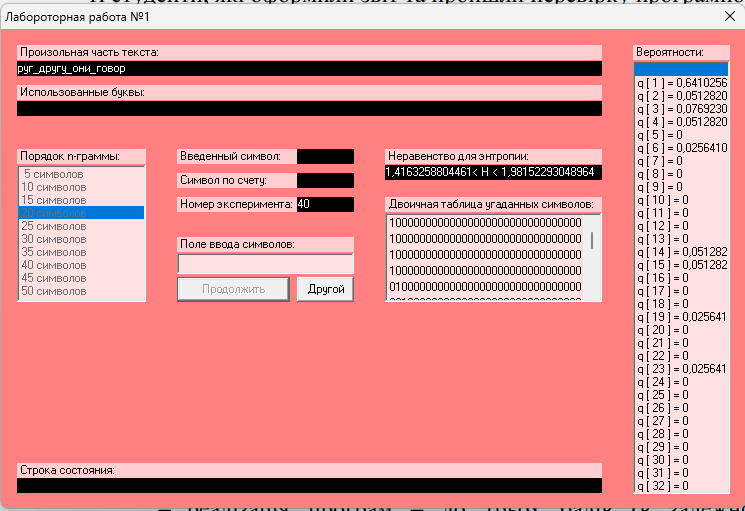
\includegraphics[scale=0.6]{Ентропія 20-грами.png}
    \end{center}

    Скріншот підрахунку ентропії $H^{(30)}$:

    \begin{center}
        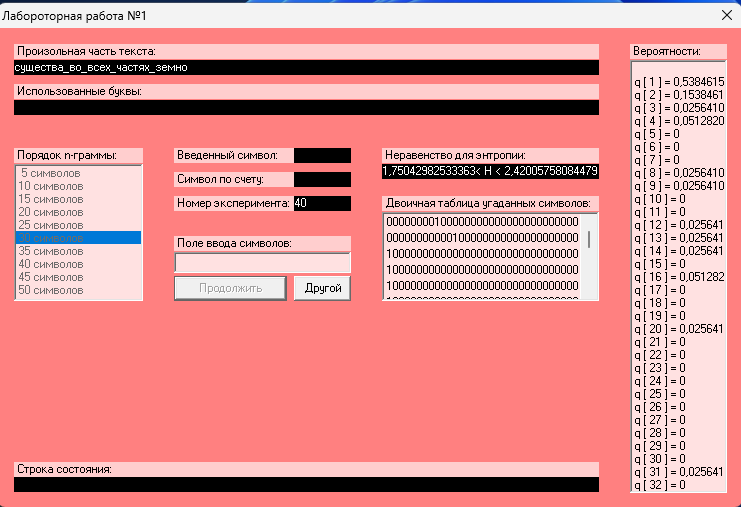
\includegraphics[scale=0.6]{Ентропія 30-грами.png}
    \end{center}

    \section{Оцінка надлишковості російської мови}

    Маємо, що:

    \begin{align*}
        1.535 \le H^{(10)} \le 2.337 \\
        1.416 \le H^{(20)} \le 1.982 \\
        1.750 \le H^{(30)} \le 2.420
    \end{align*}

    Надлишковість обчислюється за формулою:

    $$
        R = 1 - \frac{H_{\inf}}{H_0},\ \text{де}\ H_0 = \log_2 32 = 5
    $$

    Маючи ці відомості, оцінимо надлишковість:

    \begin{align*}
        H^{(10)}:\ 0.693 \geq R \geq 0.5326 \\
        H^{(20)}:\ 0.717 \geq R \geq 0.604 \\
        H^{(30)}:\ 0.65 \geq R \geq 0.516
    \end{align*}

    \section{Висновок}

    У роботі ми оцінили надлишковість російської мови та ентропії на символ та біграм,
    що певне знадобиться нам у подальших дослідженнях. Ось така штука.

    \section*{Додаток А: результат підрахунку біграм}

    \subsection*{Без пробілів}

Перетинні біграми:

\begin{verbatim}
    Overlapping Bigrams: 
    аб -- 1, 0.000869565,
    ав -- 2, 0.00173913,
    аг -- 1, 0.000869565,
    ад -- 2, 0.00173913,
    ае -- 5, 0.00434783,
    аж -- 7, 0.00608696,
    аз -- 5, 0.00434783,
    ак -- 4, 0.00347826,
    ал -- 5, 0.00434783,
    ам -- 5, 0.00434783,
    ан -- 11, 0.00956522,
    ап -- 2, 0.00173913,
    ар -- 3, 0.0026087,
    ас -- 4, 0.00347826,
    ат -- 7, 0.00608696,
    ау -- 1, 0.000869565,
    ах -- 2, 0.00173913,
    аш -- 1, 0.000869565,
    аю -- 3, 0.0026087,
    ба -- 2, 0.00173913,
    бб -- 1, 0.000869565,
    бе -- 2, 0.00173913,
    бж -- 1, 0.000869565,
    би -- 1, 0.000869565,
    бл -- 1, 0.000869565,
    бо -- 5, 0.00434783,
    бр -- 2, 0.00173913,
    бх -- 1, 0.000869565,
    бы -- 1, 0.000869565,
    бя -- 2, 0.00173913,
    ва -- 10, 0.00869565,
    вд -- 3, 0.0026087,
    ве -- 7, 0.00608696,
    ви -- 7, 0.00608696,
    вк -- 1, 0.000869565,
    вл -- 1, 0.000869565,
    вм -- 1, 0.000869565,
    вн -- 4, 0.00347826,
    во -- 15, 0.0130435,
    вс -- 3, 0.0026087,
    ву -- 1, 0.000869565,
    вы -- 8, 0.00695652,
    вь -- 1, 0.000869565,
    га -- 4, 0.00347826,
    гд -- 1, 0.000869565,
    ги -- 1, 0.000869565,
    гк -- 1, 0.000869565,
    гл -- 1, 0.000869565,
    го -- 4, 0.00347826,
    гр -- 2, 0.00173913,
    гс -- 1, 0.000869565,
    гт -- 1, 0.000869565,
    гу -- 2, 0.00173913,
    да -- 3, 0.0026087,
    дв -- 1, 0.000869565,
    дд -- 1, 0.000869565,
    де -- 7, 0.00608696,
    ди -- 4, 0.00347826,
    дн -- 1, 0.000869565,
    до -- 7, 0.00608696,
    др -- 2, 0.00173913,
    ду -- 1, 0.000869565,
    ды -- 3, 0.0026087,
    дь -- 1, 0.000869565,
    еа -- 1, 0.000869565,
    еб -- 4, 0.00347826,
    ев -- 6, 0.00521739,
    ег -- 3, 0.0026087,
    ед -- 2, 0.00173913,
    ее -- 3, 0.0026087,
    еж -- 1, 0.000869565,
    ез -- 1, 0.000869565,
    еи -- 8, 0.00695652,
    ей -- 4, 0.00347826,
    ек -- 1, 0.000869565,
    ел -- 7, 0.00608696,
    ем -- 10, 0.00869565,
    ен -- 15, 0.0130435,
    ео -- 3, 0.0026087,
    еп -- 3, 0.0026087,
    ер -- 9, 0.00782609,
    ес -- 8, 0.00695652,
    ет -- 5, 0.00434783,
    еу -- 2, 0.00173913,
    ех -- 2, 0.00173913,
    жд -- 3, 0.0026087,
    же -- 5, 0.00434783,
    жи -- 3, 0.0026087,
    жн -- 7, 0.00608696,
    за -- 1, 0.000869565,
    зв -- 4, 0.00347826,
    зд -- 1, 0.000869565,
    зи -- 2, 0.00173913,
    зм -- 3, 0.0026087,
    зн -- 5, 0.00434783,
    зо -- 1, 0.000869565,
    зу -- 1, 0.000869565,
    иа -- 1, 0.000869565,
    иб -- 1, 0.000869565,
    ив -- 9, 0.00782609,
    иг -- 2, 0.00173913,
    ид -- 3, 0.0026087,
    ие -- 6, 0.00521739,
    иж -- 4, 0.00347826,
    из -- 5, 0.00434783,
    ии -- 7, 0.00608696,
    ик -- 4, 0.00347826,
    ил -- 2, 0.00173913,
    им -- 12, 0.0104348,
    ин -- 4, 0.00347826,
    ио -- 3, 0.0026087,
    ип -- 3, 0.0026087,
    ир -- 4, 0.00347826,
    ис -- 7, 0.00608696,
    ит -- 12, 0.0104348,
    иу -- 2, 0.00173913,
    их -- 4, 0.00347826,
    иц -- 1, 0.000869565,
    ич -- 6, 0.00521739,
    иэ -- 1, 0.000869565,
    ию -- 1, 0.000869565,
    ия -- 8, 0.00695652,
    йв -- 1, 0.000869565,
    йд -- 1, 0.000869565,
    йж -- 1, 0.000869565,
    йи -- 1, 0.000869565,
    йк -- 1, 0.000869565,
    йм -- 1, 0.000869565,
    йп -- 1, 0.000869565,
    йс -- 1, 0.000869565,
    йч -- 1, 0.000869565,
    ка -- 5, 0.00434783,
    кг -- 1, 0.000869565,
    кж -- 1, 0.000869565,
    ки -- 4, 0.00347826,
    кл -- 3, 0.0026087,
    ко -- 6, 0.00521739,
    кр -- 6, 0.00521739,
    кс -- 1, 0.000869565,
    ку -- 1, 0.000869565,
    кф -- 1, 0.000869565,
    ла -- 7, 0.00608696,
    ле -- 4, 0.00347826,
    ли -- 5, 0.00434783,
    лк -- 1, 0.000869565,
    лн -- 2, 0.00173913,
    ло -- 1, 0.000869565,
    лу -- 1, 0.000869565,
    ль -- 8, 0.00695652,
    лю -- 1, 0.000869565,
    ля -- 3, 0.0026087,
    ма -- 3, 0.0026087,
    мб -- 1, 0.000869565,
    мг -- 1, 0.000869565,
    ме -- 8, 0.00695652,
    ми -- 6, 0.00521739,
    мк -- 1, 0.000869565,
    мн -- 3, 0.0026087,
    мо -- 12, 0.0104348,
    мп -- 1, 0.000869565,
    мр -- 2, 0.00173913,
    мс -- 3, 0.0026087,
    му -- 4, 0.00347826,
    мч -- 2, 0.00173913,
    мы -- 4, 0.00347826,
    на -- 9, 0.00782609,
    нв -- 1, 0.000869565,
    не -- 8, 0.00695652,
    ни -- 21, 0.0182609,
    нн -- 4, 0.00347826,
    но -- 27, 0.0234783,
    нс -- 2, 0.00173913,
    ну -- 1, 0.000869565,
    нц -- 1, 0.000869565,
    ны -- 4, 0.00347826,
    нь -- 2, 0.00173913,
    ня -- 3, 0.0026087,
    об -- 6, 0.00521739,
    ов -- 18, 0.0156522,
    ог -- 7, 0.00608696,
    од -- 6, 0.00521739,
    ое -- 2, 0.00173913,
    ож -- 2, 0.00173913,
    оз -- 4, 0.00347826,
    ои -- 7, 0.00608696,
    ой -- 3, 0.0026087,
    ок -- 2, 0.00173913,
    ол -- 9, 0.00782609,
    ом -- 11, 0.00956522,
    он -- 5, 0.00434783,
    оо -- 3, 0.0026087,
    оп -- 2, 0.00173913,
    ор -- 4, 0.00347826,
    ос -- 16, 0.013913,
    от -- 7, 0.00608696,
    оу -- 2, 0.00173913,
    ох -- 3, 0.0026087,
    оц -- 2, 0.00173913,
    оч -- 1, 0.000869565,
    оя -- 3, 0.0026087,
    пе -- 4, 0.00347826,
    по -- 11, 0.00956522,
    пр -- 7, 0.00608696,
    пс -- 1, 0.000869565,
    пт -- 1, 0.000869565,
    пы -- 1, 0.000869565,
    ра -- 13, 0.0113043,
    рв -- 1, 0.000869565,
    ре -- 10, 0.00869565,
    рж -- 1, 0.000869565,
    ри -- 7, 0.00608696,
    рм -- 1, 0.000869565,
    рн -- 1, 0.000869565,
    ро -- 7, 0.00608696,
    ру -- 4, 0.00347826,
    ры -- 5, 0.00434783,
    ря -- 1, 0.000869565,
    са -- 3, 0.0026087,
    св -- 6, 0.00521739,
    се -- 5, 0.00434783,
    си -- 5, 0.00434783,
    ск -- 4, 0.00347826,
    см -- 1, 0.000869565,
    со -- 3, 0.0026087,
    сп -- 5, 0.00434783,
    ср -- 1, 0.000869565,
    ст -- 18, 0.0156522,
    су -- 2, 0.00173913,
    сч -- 1, 0.000869565,
    ся -- 8, 0.00695652,
    та -- 7, 0.00608696,
    тб -- 1, 0.000869565,
    тв -- 2, 0.00173913,
    тд -- 1, 0.000869565,
    те -- 5, 0.00434783,
    ти -- 13, 0.0113043,
    тк -- 3, 0.0026087,
    тл -- 2, 0.00173913,
    тн -- 4, 0.00347826,
    то -- 12, 0.0104348,
    тп -- 2, 0.00173913,
    тр -- 3, 0.0026087,
    ть -- 19, 0.0165217,
    уб -- 1, 0.000869565,
    ув -- 2, 0.00173913,
    уг -- 3, 0.0026087,
    уд -- 4, 0.00347826,
    уз -- 2, 0.00173913,
    ул -- 2, 0.00173913,
    ум -- 1, 0.000869565,
    ун -- 1, 0.000869565,
    ур -- 1, 0.000869565,
    ус -- 3, 0.0026087,
    ут -- 2, 0.00173913,
    уч -- 1, 0.000869565,
    ущ -- 1, 0.000869565,
    ую -- 2, 0.00173913,
    фи -- 1, 0.000869565,
    ха -- 1, 0.000869565,
    хв -- 1, 0.000869565,
    хи -- 1, 0.000869565,
    хн -- 4, 0.00347826,
    хо -- 5, 0.00434783,
    хр -- 1, 0.000869565,
    хс -- 2, 0.00173913,
    це -- 2, 0.00173913,
    ци -- 2, 0.00173913,
    ча -- 1, 0.000869565,
    че -- 5, 0.00434783,
    чи -- 1, 0.000869565,
    чн -- 3, 0.0026087,
    чт -- 3, 0.0026087,
    чь -- 1, 0.000869565,
    ше -- 2, 0.00173913,
    ще -- 2, 0.00173913,
    ыв -- 1, 0.000869565,
    ыд -- 2, 0.00173913,
    ые -- 6, 0.00521739,
    ыз -- 1, 0.000869565,
    ыи -- 1, 0.000869565,
    ый -- 2, 0.00173913,
    ык -- 1, 0.000869565,
    ым -- 3, 0.0026087,
    ыс -- 1, 0.000869565,
    ыт -- 4, 0.00347826,
    ыу -- 1, 0.000869565,
    ых -- 2, 0.00173913,
    ыэ -- 1, 0.000869565,
    ьб -- 1, 0.000869565,
    ьв -- 5, 0.00434783,
    ьд -- 1, 0.000869565,
    ьи -- 1, 0.000869565,
    ьк -- 1, 0.000869565,
    ьн -- 8, 0.00695652,
    ьп -- 3, 0.0026087,
    ьс -- 7, 0.00608696,
    ьт -- 1, 0.000869565,
    ьч -- 1, 0.000869565,
    ьш -- 1, 0.000869565,
    ьэ -- 1, 0.000869565,
    ью -- 1, 0.000869565,
    эм -- 1, 0.000869565,
    эт -- 2, 0.00173913,
    юк -- 1, 0.000869565,
    юр -- 2, 0.00173913,
    ют -- 4, 0.00347826,
    юч -- 1, 0.000869565,
    ющ -- 1, 0.000869565,
    яб -- 2, 0.00173913,
    яв -- 2, 0.00173913,
    яи -- 3, 0.0026087,
    як -- 3, 0.0026087,
    ям -- 1, 0.000869565,
    ян -- 1, 0.000869565,
    яп -- 3, 0.0026087,
    яр -- 1, 0.000869565,
    яс -- 2, 0.00173913,
    ят -- 7, 0.00608696,
    ях -- 1, 0.000869565,
    яю -- 1, 0.000869565,
    Total overlaping bigrams in text: 1150
    Entropy of overlaping bigrams in text: 3.88691
    
\end{verbatim}

Неперетинні біграми:

\begin{verbatim}
    ав -- 1, 0.00173913,
    ае -- 2, 0.00347826,
    аж -- 3, 0.00521739,
    аз -- 2, 0.00347826,
    ал -- 2, 0.00347826,
    ам -- 3, 0.00521739,
    ан -- 4, 0.00695652,
    ар -- 2, 0.00347826,
    ас -- 3, 0.00521739,
    ат -- 3, 0.00521739,
    ау -- 1, 0.00173913,
    аш -- 1, 0.00173913,
    ба -- 1, 0.00173913,
    бж -- 1, 0.00173913,
    би -- 1, 0.00173913,
    бо -- 3, 0.00521739,
    бр -- 1, 0.00173913,
    бя -- 1, 0.00173913,
    ва -- 6, 0.0104348,
    вд -- 3, 0.00521739,
    ве -- 5, 0.00869565,
    ви -- 3, 0.00521739,
    вк -- 1, 0.00173913,
    вл -- 1, 0.00173913,
    вн -- 3, 0.00521739,
    во -- 11, 0.0191304,
    вс -- 2, 0.00347826,
    вы -- 6, 0.0104348,
    га -- 2, 0.00347826,
    ги -- 1, 0.00173913,
    гк -- 1, 0.00173913,
    го -- 3, 0.00521739,
    да -- 3, 0.00521739,
    дв -- 1, 0.00173913,
    дд -- 1, 0.00173913,
    де -- 4, 0.00695652,
    ди -- 2, 0.00347826,
    дн -- 1, 0.00173913,
    до -- 1, 0.00173913,
    др -- 1, 0.00173913,
    ду -- 1, 0.00173913,
    ды -- 1, 0.00173913,
    дь -- 1, 0.00173913,
    еа -- 1, 0.00173913,
    еб -- 3, 0.00521739,
    ев -- 1, 0.00173913,
    ег -- 2, 0.00347826,
    ед -- 1, 0.00173913,
    ее -- 2, 0.00347826,
    еж -- 1, 0.00173913,
    ез -- 1, 0.00173913,
    еи -- 5, 0.00869565,
    ей -- 3, 0.00521739,
    ел -- 2, 0.00347826,
    ем -- 4, 0.00695652,
    ен -- 6, 0.0104348,
    ео -- 2, 0.00347826,
    еп -- 2, 0.00347826,
    ер -- 8, 0.013913,
    ес -- 5, 0.00869565,
    ет -- 4, 0.00695652,
    еу -- 1, 0.00173913,
    ех -- 2, 0.00347826,
    жд -- 2, 0.00347826,
    же -- 3, 0.00521739,
    жи -- 2, 0.00347826,
    жн -- 3, 0.00521739,
    за -- 1, 0.00173913,
    зв -- 2, 0.00347826,
    зд -- 1, 0.00173913,
    зи -- 1, 0.00173913,
    зм -- 1, 0.00173913,
    зн -- 2, 0.00347826,
    зо -- 1, 0.00173913,
    ив -- 2, 0.00347826,
    иг -- 2, 0.00347826,
    ид -- 2, 0.00347826,
    ие -- 4, 0.00695652,
    иж -- 1, 0.00173913,
    из -- 3, 0.00521739,
    ии -- 2, 0.00347826,
    им -- 6, 0.0104348,
    ин -- 2, 0.00347826,
    ио -- 2, 0.00347826,
    ип -- 1, 0.00173913,
    ир -- 2, 0.00347826,
    ис -- 4, 0.00695652,
    ит -- 7, 0.0121739,
    иу -- 1, 0.00173913,
    их -- 3, 0.00521739,
    иц -- 1, 0.00173913,
    ич -- 4, 0.00695652,
    йи -- 1, 0.00173913,
    йм -- 1, 0.00173913,
    йп -- 1, 0.00173913,
    ка -- 5, 0.00869565,
    кг -- 1, 0.00173913,
    кж -- 1, 0.00173913,
    ки -- 3, 0.00521739,
    кл -- 2, 0.00347826,
    ко -- 3, 0.00521739,
    кр -- 4, 0.00695652,
    кс -- 1, 0.00173913,
    ку -- 1, 0.00173913,
    кф -- 1, 0.00173913,
    ла -- 6, 0.0104348,
    ле -- 3, 0.00521739,
    ли -- 3, 0.00521739,
    лн -- 2, 0.00347826,
    ло -- 1, 0.00173913,
    лу -- 1, 0.00173913,
    ль -- 5, 0.00869565,
    ля -- 1, 0.00173913,
    ма -- 1, 0.00173913,
    мг -- 1, 0.00173913,
    ме -- 3, 0.00521739,
    ми -- 4, 0.00695652,
    мо -- 6, 0.0104348,
    мр -- 2, 0.00347826,
    мс -- 3, 0.00521739,
    му -- 4, 0.00695652,
    мч -- 1, 0.00173913,
    мы -- 2, 0.00347826,
    на -- 5, 0.00869565,
    не -- 4, 0.00695652,
    ни -- 14, 0.0243478,
    нн -- 1, 0.00173913,
    но -- 17, 0.0295652,
    нс -- 1, 0.00173913,
    ны -- 3, 0.00521739,
    нь -- 2, 0.00347826,
    ня -- 2, 0.00347826,
    об -- 6, 0.0104348,
    ов -- 5, 0.00869565,
    ог -- 3, 0.00521739,
    од -- 1, 0.00173913,
    ое -- 1, 0.00173913,
    ож -- 1, 0.00173913,
    оз -- 2, 0.00347826,
    ои -- 2, 0.00347826,
    ой -- 1, 0.00173913,
    ол -- 2, 0.00347826,
    ом -- 5, 0.00869565,
    он -- 3, 0.00521739,
    оо -- 1, 0.00173913,
    оп -- 2, 0.00347826,
    ор -- 3, 0.00521739,
    ос -- 9, 0.0156522,
    от -- 3, 0.00521739,
    оу -- 1, 0.00173913,
    ох -- 2, 0.00347826,
    оц -- 2, 0.00347826,
    оч -- 1, 0.00173913,
    оя -- 1, 0.00173913,
    по -- 5, 0.00869565,
    пр -- 5, 0.00869565,
    пс -- 1, 0.00173913,
    пт -- 1, 0.00173913,
    пы -- 1, 0.00173913,
    ра -- 6, 0.0104348,
    рв -- 1, 0.00173913,
    ре -- 2, 0.00347826,
    ри -- 2, 0.00347826,
    ро -- 3, 0.00521739,
    ру -- 2, 0.00347826,
    ры -- 2, 0.00347826,
    ря -- 1, 0.00173913,
    са -- 1, 0.00173913,
    св -- 2, 0.00347826,
    се -- 2, 0.00347826,
    си -- 3, 0.00521739,
    см -- 1, 0.00173913,
    со -- 2, 0.00347826,
    сп -- 4, 0.00695652,
    ср -- 1, 0.00173913,
    ст -- 6, 0.0104348,
    су -- 1, 0.00173913,
    ся -- 4, 0.00695652,
    та -- 5, 0.00869565,
    те -- 2, 0.00347826,
    ти -- 10, 0.0173913,
    тк -- 2, 0.00347826,
    тн -- 1, 0.00173913,
    то -- 4, 0.00695652,
    тр -- 1, 0.00173913,
    ть -- 10, 0.0173913,
    ув -- 2, 0.00347826,
    уг -- 2, 0.00347826,
    уд -- 1, 0.00173913,
    уз -- 1, 0.00173913,
    ул -- 2, 0.00347826,
    ут -- 1, 0.00173913,
    уч -- 1, 0.00173913,
    ую -- 2, 0.00347826,
    хн -- 1, 0.00173913,
    хо -- 3, 0.00521739,
    хр -- 1, 0.00173913,
    хс -- 1, 0.00173913,
    ци -- 1, 0.00173913,
    ча -- 1, 0.00173913,
    че -- 1, 0.00173913,
    чн -- 1, 0.00173913,
    чт -- 2, 0.00347826,
    чь -- 1, 0.00173913,
    ше -- 1, 0.00173913,
    ще -- 1, 0.00173913,
    ыв -- 1, 0.00173913,
    ыд -- 1, 0.00173913,
    ые -- 2, 0.00347826,
    ыи -- 1, 0.00173913,
    ый -- 2, 0.00347826,
    ым -- 1, 0.00173913,
    ыс -- 1, 0.00173913,
    ыт -- 1, 0.00173913,
    ых -- 1, 0.00173913,
    ьб -- 1, 0.00173913,
    ьв -- 1, 0.00173913,
    ьд -- 1, 0.00173913,
    ьк -- 1, 0.00173913,
    ьн -- 3, 0.00521739,
    ьс -- 4, 0.00695652,
    ьт -- 1, 0.00173913,
    ью -- 1, 0.00173913,
    эм -- 1, 0.00173913,
    эт -- 2, 0.00347826,
    ют -- 4, 0.00695652,
    юч -- 1, 0.00173913,
    ющ -- 1, 0.00173913,
    яб -- 1, 0.00173913,
    яв -- 2, 0.00347826,
    яи -- 2, 0.00347826,
    як -- 2, 0.00347826,
    ям -- 1, 0.00173913,
    ян -- 1, 0.00173913,
    яп -- 2, 0.00347826,
    яр -- 1, 0.00173913,
    ят -- 4, 0.00695652,
    ях -- 1, 0.00173913,
    Total non overlaping bigrams in text: 575
    Entropy of non overlaping bigrams in text: 3.74531
    
\end{verbatim}


\subsection*{З пробілами}

Перетинні біграми:

\begin{verbatim}
    а -- 1, 0.000743494,
    б -- 8, 0.00594796,
    в -- 25, 0.0185874,
    г -- 2, 0.00148699,
    д -- 6, 0.00446097,
    ж -- 3, 0.00223048,
    з -- 2, 0.00148699,
    и -- 26, 0.0193309,
    к -- 10, 0.00743494,
    л -- 3, 0.00223048,
    м -- 8, 0.00594796,
    н -- 17, 0.0126394,
    о -- 5, 0.00371747,
    п -- 19, 0.0141264,
    р -- 11, 0.00817844,
    с -- 23, 0.0171004,
    т -- 6, 0.00446097,
    у -- 9, 0.00669145,
    ф -- 1, 0.000743494,
    х -- 1, 0.000743494,
    ц -- 1, 0.000743494,
    ч -- 5, 0.00371747,
    э -- 3, 0.00223048,
   а  -- 4, 0.00297398,
   аб -- 1, 0.000743494,
   ав -- 2, 0.00148699,
   аг -- 1, 0.000743494,
   ад -- 2, 0.00148699,
   ае -- 5, 0.00371747,
   аж -- 7, 0.00520446,
   аз -- 5, 0.00371747,
   ак -- 4, 0.00297398,
   ал -- 5, 0.00371747,
   ам -- 5, 0.00371747,
   ан -- 11, 0.00817844,
   ап -- 1, 0.000743494,
   ар -- 2, 0.00148699,
   ас -- 3, 0.00223048,
   ат -- 7, 0.00520446,
   ах -- 2, 0.00148699,
   аш -- 1, 0.000743494,
   аю -- 3, 0.00223048,
   ба -- 2, 0.00148699,
   бб -- 1, 0.000743494,
   бе -- 2, 0.00148699,
   бж -- 1, 0.000743494,
   би -- 1, 0.000743494,
   бл -- 1, 0.000743494,
   бо -- 5, 0.00371747,
   бр -- 2, 0.00148699,
   бх -- 1, 0.000743494,
   бы -- 1, 0.000743494,
   бя -- 2, 0.00148699,
   в  -- 4, 0.00297398,
   ва -- 10, 0.00743494,
   вд -- 2, 0.00148699,
   ве -- 7, 0.00520446,
   ви -- 7, 0.00520446,
   вк -- 1, 0.000743494,
   вл -- 1, 0.000743494,
   вн -- 3, 0.00223048,
   во -- 15, 0.0111524,
   вс -- 2, 0.00148699,
   ву -- 1, 0.000743494,
   вы -- 8, 0.00594796,
   вь -- 1, 0.000743494,
   г  -- 2, 0.00148699,
   га -- 4, 0.00297398,
   гд -- 1, 0.000743494,
   ги -- 1, 0.000743494,
   гк -- 1, 0.000743494,
   гл -- 1, 0.000743494,
   го -- 4, 0.00297398,
   гр -- 2, 0.00148699,
   гу -- 2, 0.00148699,
   д  -- 1, 0.000743494,
   да -- 3, 0.00223048,
   дд -- 1, 0.000743494,
   де -- 7, 0.00520446,
   ди -- 4, 0.00297398,
   дн -- 1, 0.000743494,
   до -- 7, 0.00520446,
   др -- 2, 0.00148699,
   ду -- 1, 0.000743494,
   ды -- 3, 0.00223048,
   дь -- 1, 0.000743494,
   е  -- 27, 0.0200743,
   еб -- 3, 0.00223048,
   ев -- 2, 0.00148699,
   ег -- 3, 0.00223048,
   ед -- 2, 0.00148699,
   ее -- 3, 0.00223048,
   еж -- 1, 0.000743494,
   ез -- 1, 0.000743494,
   еи -- 1, 0.000743494,
   ей -- 4, 0.00297398,
   ек -- 1, 0.000743494,
   ел -- 6, 0.00446097,
   ем -- 9, 0.00669145,
   ен -- 15, 0.0111524,
   ео -- 2, 0.00148699,
   ер -- 7, 0.00520446,
   ес -- 6, 0.00446097,
   ет -- 3, 0.00223048,
   ех -- 2, 0.00148699,
   жд -- 3, 0.00223048,
   же -- 5, 0.00371747,
   жи -- 3, 0.00223048,
   жн -- 7, 0.00520446,
   за -- 1, 0.000743494,
   зв -- 4, 0.00297398,
   зд -- 1, 0.000743494,
   зи -- 2, 0.00148699,
   зм -- 3, 0.00223048,
   зн -- 5, 0.00371747,
   зо -- 1, 0.000743494,
   зу -- 1, 0.000743494,
   и  -- 36, 0.0267658,
   иа -- 1, 0.000743494,
   ив -- 5, 0.00371747,
   иг -- 2, 0.00148699,
   ид -- 2, 0.00148699,
   ие -- 6, 0.00446097,
   иж -- 2, 0.00148699,
   из -- 4, 0.00297398,
   ии -- 2, 0.00148699,
   ик -- 2, 0.00148699,
   ил -- 2, 0.00148699,
   им -- 9, 0.00669145,
   ин -- 2, 0.00148699,
   ио -- 1, 0.000743494,
   ир -- 3, 0.00223048,
   ис -- 3, 0.00223048,
   ит -- 12, 0.00892193,
   их -- 4, 0.00297398,
   ич -- 5, 0.00371747,
   ию -- 1, 0.000743494,
   ия -- 8, 0.00594796,
   й  -- 8, 0.00594796,
   йс -- 1, 0.000743494,
   к  -- 7, 0.00520446,
   ка -- 5, 0.00371747,
   кж -- 1, 0.000743494,
   ки -- 2, 0.00148699,
   кл -- 2, 0.00148699,
   ко -- 6, 0.00446097,
   кр -- 6, 0.00446097,
   л  -- 1, 0.000743494,
   ла -- 7, 0.00520446,
   ле -- 4, 0.00297398,
   ли -- 5, 0.00371747,
   лн -- 2, 0.00148699,
   ло -- 1, 0.000743494,
   лу -- 1, 0.000743494,
   ль -- 8, 0.00594796,
   лю -- 1, 0.000743494,
   ля -- 3, 0.00223048,
   м  -- 14, 0.0104089,
   ма -- 3, 0.00223048,
   ме -- 8, 0.00594796,
   ми -- 5, 0.00371747,
   мн -- 1, 0.000743494,
   мо -- 11, 0.00817844,
   мс -- 1, 0.000743494,
   му -- 4, 0.00297398,
   мы -- 4, 0.00297398,
   н  -- 3, 0.00223048,
   на -- 9, 0.00669145,
   не -- 8, 0.00594796,
   ни -- 19, 0.0141264,
   нн -- 4, 0.00297398,
   но -- 27, 0.0200743,
   нс -- 2, 0.00148699,
   ну -- 1, 0.000743494,
   нц -- 1, 0.000743494,
   ны -- 4, 0.00297398,
   нь -- 2, 0.00148699,
   ня -- 3, 0.00223048,
   о  -- 20, 0.0148699,
   об -- 5, 0.00371747,
   ов -- 15, 0.0111524,
   ог -- 7, 0.00520446,
   од -- 6, 0.00446097,
   ое -- 2, 0.00148699,
   ож -- 2, 0.00148699,
   оз -- 4, 0.00297398,
   ои -- 4, 0.00297398,
   ой -- 3, 0.00223048,
   ок -- 2, 0.00148699,
   ол -- 9, 0.00669145,
   ом -- 10, 0.00743494,
   он -- 4, 0.00297398,
   оо -- 2, 0.00148699,
   ор -- 3, 0.00223048,
   ос -- 12, 0.00892193,
   от -- 6, 0.00446097,
   ох -- 3, 0.00223048,
   оц -- 2, 0.00148699,
   оч -- 1, 0.000743494,
   оя -- 3, 0.00223048,
   пе -- 4, 0.00297398,
   по -- 11, 0.00817844,
   пр -- 7, 0.00520446,
   пс -- 1, 0.000743494,
   пт -- 1, 0.000743494,
   пы -- 1, 0.000743494,
   р  -- 1, 0.000743494,
   ра -- 13, 0.00966543,
   ре -- 10, 0.00743494,
   рж -- 1, 0.000743494,
   ри -- 7, 0.00520446,
   рм -- 1, 0.000743494,
   рн -- 1, 0.000743494,
   ро -- 7, 0.00520446,
   ру -- 4, 0.00297398,
   ры -- 5, 0.00371747,
   ря -- 1, 0.000743494,
   с  -- 1, 0.000743494,
   са -- 3, 0.00223048,
   св -- 6, 0.00446097,
   се -- 5, 0.00371747,
   си -- 5, 0.00371747,
   ск -- 4, 0.00297398,
   со -- 3, 0.00223048,
   сп -- 5, 0.00371747,
   ср -- 1, 0.000743494,
   ст -- 18, 0.0133829,
   су -- 2, 0.00148699,
   сч -- 1, 0.000743494,
   ся -- 8, 0.00594796,
   т  -- 10, 0.00743494,
   та -- 7, 0.00520446,
   тв -- 1, 0.000743494,
   тд -- 1, 0.000743494,
   те -- 5, 0.00371747,
   ти -- 13, 0.00966543,
   тк -- 2, 0.00148699,
   тл -- 1, 0.000743494,
   тн -- 1, 0.000743494,
   то -- 12, 0.00892193,
   тр -- 2, 0.00148699,
   ть -- 19, 0.0141264,
   у  -- 5, 0.00371747,
   уб -- 1, 0.000743494,
   ув -- 1, 0.000743494,
   уг -- 3, 0.00223048,
   уд -- 4, 0.00297398,
   уз -- 1, 0.000743494,
   ул -- 2, 0.00148699,
   ум -- 1, 0.000743494,
   ун -- 1, 0.000743494,
   ус -- 2, 0.00148699,
   ут -- 1, 0.000743494,
   уч -- 1, 0.000743494,
   ущ -- 1, 0.000743494,
   ую -- 2, 0.00148699,
   фи -- 1, 0.000743494,
   х  -- 5, 0.00371747,
   ха -- 1, 0.000743494,
   хи -- 1, 0.000743494,
   хн -- 2, 0.00148699,
   хо -- 5, 0.00371747,
   хр -- 1, 0.000743494,
   це -- 2, 0.00148699,
   ци -- 2, 0.00148699,
   ча -- 1, 0.000743494,
   че -- 5, 0.00371747,
   чи -- 1, 0.000743494,
   чн -- 3, 0.00223048,
   чт -- 3, 0.00223048,
   чь -- 1, 0.000743494,
   ше -- 2, 0.00148699,
   ще -- 2, 0.00148699,
   ы  -- 6, 0.00446097,
   ыв -- 1, 0.000743494,
   ые -- 6, 0.00446097,
   ыз -- 1, 0.000743494,
   ый -- 2, 0.00148699,
   ык -- 1, 0.000743494,
   ым -- 3, 0.00223048,
   ыт -- 4, 0.00297398,
   ых -- 2, 0.00148699,
   ь  -- 19, 0.0141264,
   ьк -- 1, 0.000743494,
   ьн -- 3, 0.00223048,
   ьс -- 6, 0.00446097,
   ьт -- 1, 0.000743494,
   ьш -- 1, 0.000743494,
   ью -- 1, 0.000743494,
   эм -- 1, 0.000743494,
   эт -- 2, 0.00148699,
   ю  -- 4, 0.00297398,
   ют -- 3, 0.00223048,
   юч -- 1, 0.000743494,
   ющ -- 1, 0.000743494,
   я  -- 17, 0.0126394,
   ям -- 1, 0.000743494,
   яр -- 1, 0.000743494,
   ят -- 7, 0.00520446,
   яю -- 1, 0.000743494,
   Total overlaping bigrams in text: 1345
   Entropy of overlaping bigrams in text: 3.78871
   
\end{verbatim}

Непертинні біграми:

\begin{verbatim}
    б -- 5, 0.00742942,
    в -- 14, 0.0208024,
    г -- 1, 0.00148588,
    д -- 4, 0.00594354,
    и -- 14, 0.0208024,
    к -- 7, 0.0104012,
    л -- 2, 0.00297177,
    м -- 4, 0.00594354,
    н -- 6, 0.0089153,
    о -- 3, 0.00445765,
    п -- 11, 0.0163447,
    р -- 3, 0.00445765,
    с -- 9, 0.013373,
    т -- 1, 0.00148588,
    у -- 6, 0.0089153,
    ф -- 1, 0.00148588,
    ц -- 1, 0.00148588,
    ч -- 2, 0.00297177,
   а  -- 2, 0.00297177,
   аг -- 1, 0.00148588,
   ад -- 2, 0.00297177,
   ае -- 3, 0.00445765,
   аж -- 4, 0.00594354,
   аз -- 1, 0.00148588,
   ак -- 3, 0.00445765,
   ал -- 1, 0.00148588,
   ам -- 1, 0.00148588,
   ан -- 7, 0.0104012,
   ап -- 1, 0.00148588,
   ар -- 2, 0.00297177,
   ас -- 1, 0.00148588,
   ат -- 3, 0.00445765,
   ах -- 1, 0.00148588,
   аю -- 2, 0.00297177,
   ба -- 1, 0.00148588,
   бб -- 1, 0.00148588,
   бл -- 1, 0.00148588,
   бо -- 2, 0.00297177,
   бр -- 1, 0.00148588,
   бх -- 1, 0.00148588,
   бя -- 1, 0.00148588,
   в  -- 2, 0.00297177,
   ва -- 4, 0.00594354,
   вд -- 1, 0.00148588,
   ве -- 4, 0.00594354,
   ви -- 1, 0.00148588,
   вн -- 2, 0.00297177,
   во -- 7, 0.0104012,
   вс -- 1, 0.00148588,
   ву -- 1, 0.00148588,
   вы -- 4, 0.00594354,
   г  -- 1, 0.00148588,
   га -- 1, 0.00148588,
   ги -- 1, 0.00148588,
   гк -- 1, 0.00148588,
   гл -- 1, 0.00148588,
   го -- 3, 0.00445765,
   гр -- 1, 0.00148588,
   гу -- 1, 0.00148588,
   да -- 1, 0.00148588,
   де -- 2, 0.00297177,
   ди -- 2, 0.00297177,
   до -- 3, 0.00445765,
   др -- 1, 0.00148588,
   ды -- 2, 0.00297177,
   е  -- 12, 0.0178306,
   еб -- 2, 0.00297177,
   ег -- 1, 0.00148588,
   ед -- 2, 0.00297177,
   ее -- 2, 0.00297177,
   еи -- 1, 0.00148588,
   ей -- 2, 0.00297177,
   ек -- 1, 0.00148588,
   ел -- 4, 0.00594354,
   ем -- 3, 0.00445765,
   ен -- 5, 0.00742942,
   ео -- 2, 0.00297177,
   ер -- 4, 0.00594354,
   ес -- 3, 0.00445765,
   ет -- 2, 0.00297177,
   ех -- 1, 0.00148588,
   жд -- 2, 0.00297177,
   же -- 4, 0.00594354,
   жи -- 2, 0.00297177,
   жн -- 2, 0.00297177,
   за -- 1, 0.00148588,
   зв -- 4, 0.00594354,
   зд -- 1, 0.00148588,
   зм -- 3, 0.00445765,
   зн -- 4, 0.00594354,
   зу -- 1, 0.00148588,
   и  -- 21, 0.0312036,
   иа -- 1, 0.00148588,
   ив -- 2, 0.00297177,
   иг -- 1, 0.00148588,
   ид -- 2, 0.00297177,
   ие -- 5, 0.00742942,
   из -- 1, 0.00148588,
   ик -- 1, 0.00148588,
   им -- 7, 0.0104012,
   ин -- 1, 0.00148588,
   ио -- 1, 0.00148588,
   ир -- 1, 0.00148588,
   ис -- 2, 0.00297177,
   ит -- 6, 0.0089153,
   ич -- 4, 0.00594354,
   ия -- 4, 0.00594354,
   й  -- 4, 0.00594354,
   йс -- 1, 0.00148588,
   к  -- 1, 0.00148588,
   ка -- 2, 0.00297177,
   кж -- 1, 0.00148588,
   ки -- 1, 0.00148588,
   кл -- 1, 0.00148588,
   ко -- 3, 0.00445765,
   кр -- 3, 0.00445765,
   л  -- 1, 0.00148588,
   ла -- 3, 0.00445765,
   ле -- 3, 0.00445765,
   ли -- 1, 0.00148588,
   лн -- 2, 0.00297177,
   ль -- 7, 0.0104012,
   лю -- 1, 0.00148588,
   ля -- 2, 0.00297177,
   м  -- 11, 0.0163447,
   ме -- 3, 0.00445765,
   ми -- 2, 0.00297177,
   мо -- 3, 0.00445765,
   му -- 2, 0.00297177,
   мы -- 2, 0.00297177,
   н  -- 1, 0.00148588,
   на -- 5, 0.00742942,
   не -- 5, 0.00742942,
   ни -- 10, 0.0148588,
   нн -- 2, 0.00297177,
   но -- 18, 0.0267459,
   нс -- 1, 0.00148588,
   нц -- 1, 0.00148588,
   ны -- 2, 0.00297177,
   нь -- 1, 0.00148588,
   ня -- 2, 0.00297177,
   о  -- 6, 0.0089153,
   об -- 2, 0.00297177,
   ов -- 9, 0.013373,
   ог -- 3, 0.00445765,
   од -- 4, 0.00594354,
   ож -- 2, 0.00297177,
   ои -- 3, 0.00445765,
   ой -- 1, 0.00148588,
   ок -- 1, 0.00148588,
   ол -- 3, 0.00445765,
   ом -- 7, 0.0104012,
   он -- 1, 0.00148588,
   оо -- 2, 0.00297177,
   ор -- 2, 0.00297177,
   ос -- 4, 0.00594354,
   от -- 3, 0.00445765,
   ох -- 2, 0.00297177,
   оц -- 2, 0.00297177,
   оя -- 2, 0.00297177,
   пе -- 1, 0.00148588,
   по -- 5, 0.00742942,
   пр -- 4, 0.00594354,
   ра -- 10, 0.0148588,
   ре -- 5, 0.00742942,
   рж -- 1, 0.00148588,
   ри -- 3, 0.00445765,
   рн -- 1, 0.00148588,
   ро -- 3, 0.00445765,
   ру -- 2, 0.00297177,
   ры -- 2, 0.00297177,
   с  -- 1, 0.00148588,
   са -- 2, 0.00297177,
   св -- 4, 0.00594354,
   се -- 2, 0.00297177,
   си -- 4, 0.00594354,
   ск -- 2, 0.00297177,
   со -- 1, 0.00148588,
   сп -- 3, 0.00445765,
   ср -- 1, 0.00148588,
   ст -- 12, 0.0178306,
   ся -- 6, 0.0089153,
   т  -- 5, 0.00742942,
   та -- 3, 0.00445765,
   тв -- 1, 0.00148588,
   те -- 3, 0.00445765,
   ти -- 5, 0.00742942,
   тк -- 1, 0.00148588,
   то -- 7, 0.0104012,
   тр -- 1, 0.00148588,
   ть -- 11, 0.0163447,
   у  -- 4, 0.00594354,
   уб -- 1, 0.00148588,
   уг -- 1, 0.00148588,
   уд -- 2, 0.00297177,
   уз -- 1, 0.00148588,
   ус -- 1, 0.00148588,
   ут -- 1, 0.00148588,
   ущ -- 1, 0.00148588,
   ую -- 1, 0.00148588,
   х  -- 4, 0.00594354,
   ха -- 1, 0.00148588,
   хи -- 1, 0.00148588,
   хн -- 1, 0.00148588,
   хо -- 3, 0.00445765,
   ча -- 1, 0.00148588,
   че -- 3, 0.00445765,
   чи -- 1, 0.00148588,
   чн -- 1, 0.00148588,
   чт -- 2, 0.00297177,
   ше -- 2, 0.00297177,
   ще -- 1, 0.00148588,
   ы  -- 5, 0.00742942,
   ыв -- 1, 0.00148588,
   ые -- 3, 0.00445765,
   ыз -- 1, 0.00148588,
   ый -- 1, 0.00148588,
   ым -- 1, 0.00148588,
   ыт -- 2, 0.00297177,
   ь  -- 11, 0.0163447,
   ьс -- 1, 0.00148588,
   ью -- 1, 0.00148588,
   эм -- 1, 0.00148588,
   эт -- 2, 0.00297177,
   ю  -- 2, 0.00297177,
   ют -- 1, 0.00148588,
   я  -- 7, 0.0104012,
   ям -- 1, 0.00148588,
   ят -- 2, 0.00297177,
   яю -- 1, 0.00148588,
   Total non overlaping bigrams in text: 673
   Entropy of non overlaping bigrams in text: 3.66332
   
\end{verbatim}


\end{document}